\documentclass{ieeeaccess}
\usepackage{cite}
\usepackage{graphicx}
\usepackage{amsmath,amssymb,amsfonts}
\usepackage[bahasa]{babel}

\renewcommand{\abstractname}{Abstrak}
\renewcommand{\IEEEkeywordsname}{Istilah Indeks}
\renewcommand{\refname}{DAFTAR PUSTAKA}

% ieeeaccess.cls (mirror pihak ketiga) memakai counter "biography" dan flag
% "@biographyTOCentrynotmade" di lingkungan biographynophoto tanpa pernah
% mendeklarasikannya -- deklarasikan manual di sini agar tidak error.
\newcounter{biography}
\makeatletter
\newif\if@biographyTOCentrynotmade
\@biographyTOCentrynotmadetrue
\makeatother

% \@makecaption kelas ini membandingkan \xfigwd (lebar gambar) terhadap
% \columnwidth untuk memilih gaya caption, tetapi \xfigwd hanya diisi oleh
% makro \Figure bawaan kelas -- yang tidak dipakai di sini (dipakai figure/figure*
% biasa). Deklarasikan di sini dan SELALU set ke 0pt tepat sebelum tiap \caption
% (\ifdim 0pt>\columnwidth jadi selalu FALSE) supaya dipakai cabang caption
% pendek (\raggedright polos, mengikuti \hsize konteks saat itu -- \textwidth
% di dalam figure*, \columnwidth di dalam figure -- sehingga selalu membungkus
% dengan benar). JANGAN pakai cabang "lebar" (\xfigwd=\linewidth/\textwidth):
% cabang itu memakai tabular satu baris tanpa lebar kolom sehingga TIDAK
% membungkus -- caption panjang meluber diam-diam melewati margin halaman
% tanpa error (baru ketahuan dari "Overfull \hbox" di log).
\newdimen\xfigwd

\begin{document}

\history{Date of publication xxxx 00, 0000, date of current version xxxx 00, 0000.}
\doi{10.1109/ACCESS.2017.DOI}

\title{Graph Retrieval-Augmented Generation untuk Meningkatkan Presisi \textit{Retrieval} dan Validitas Sintaksis pada Konfigurasi Kubernetes}

\author{\uppercase{Jihan Aurelia}\authorrefmark{1} and \uppercase{Dimitri Mahayana}\authorrefmark{1}}
\address[1]{School of Electrical Engineering and Informatics, Institut Teknologi Bandung, Bandung 40132, Indonesia}
\tfootnote{Naskah ini merupakan ringkasan Tugas Akhir Program Studi Sistem dan Teknologi Informasi, Institut Teknologi Bandung.}

\markboth
{Aurelia dan Mahayana: GraphRAG untuk Konfigurasi Kubernetes}
{Aurelia dan Mahayana: GraphRAG untuk Konfigurasi Kubernetes}

\corresp{Penulis koresponden: Jihan Aurelia (e-mail: 18222001@std.stei.itb.ac.id).}

\titlepgskip=-15pt

\maketitle

\begin{abstract}
Kubernetes menjadi standar de facto orkestrasi kontainer, namun kompleksitas konfigurasi YAML-nya mendorong penggunaan model bahasa besar (\textit{Large Language Model}, LLM) yang rentan menghasilkan konfigurasi keliru secara semantik. Pendekatan \textit{retrieval-augmented generation} (RAG) berbasis vektor tidak memadai karena gagal menangkap relasi hierarkis antarkomponen Kubernetes. Penelitian ini membangun sistem \textit{graph retrieval-augmented generation} (GraphRAG) yang menurunkan \textit{knowledge graph} (KG) secara deterministik dari spesifikasi OpenAPI Kubernetes, menelusurinya dengan kedalaman yang menyesuaikan \textit{intent} kueri, serta memvalidasi manifes YAML keluaran langsung terhadap graf tanpa memerlukan klaster aktif. Sistem dievaluasi terhadap \textit{Vector RAG} dan LLM tanpa konteks menggunakan 102 skenario uji yang divalidasi praktisi. Hasil menunjukkan keunggulan yang tegas pada dimensi \textit{retrieval}: skor F1 mencapai 0,71 dibanding 0,24 pada \textit{Vector RAG}, dengan selisih yang signifikan secara statistik (p$<$0,001). Penelusuran graf juga berhasil melalui sebagian besar relasi skema yang diharapkan, dengan \textit{hop accuracy} 0,76. Sebaliknya, kualitas teks jawaban tidak berbeda signifikan antarsistem, menunjukkan bahwa kontribusi \textit{knowledge graph} terletak pada ketertelusuran dan kelengkapan \textit{retrieval} struktural, bukan pada kefasihan bahasa. Temuan ini memetakan secara empiris dimensi tempat representasi graf memberi keunggulan nyata pada domain konfigurasi Kubernetes.
\end{abstract}

\begin{keywords}
graph retrieval-augmented generation, halusinasi LLM, intent-adaptive depth traversal, knowledge graph, Kubernetes, validasi YAML
\end{keywords}

\section{Pendahuluan}
\label{sec:pendahuluan}

\PARstart{K}{ubernetes} \cite{k8s_docs_concepts} telah mengukuhkan posisinya sebagai standar industri \textit{de facto} untuk orkestrasi kontainer, didorong oleh ekosistem yang matang dan fleksibilitas pengelolaan infrastruktur secara deklaratif \cite{cncf_2023_survey,gartner_cloud_2021}. Namun demikian, paradigma deklaratif ini menuntut pengembang menulis konfigurasi YAML yang verbos dan hierarkis, dengan interdependensi antarobjek yang kuat namun sering kali tidak tersurat secara eksplisit \cite{soldani_pains_2018}. Akibat kompleksitas ini, sekitar 80\% insiden operasional Kubernetes berakar pada kesalahan konfigurasi, dan 18\% berkas konfigurasi \textit{open-source} teridentifikasi mengandung kerentanan keamanan yang serius \cite{rahman2023misconfigurations}.

Situasi ini mendorong pemanfaatan LLM untuk membantu menyusun maupun menjelaskan konfigurasi Kubernetes. Akan tetapi, LLM dapat menghasilkan kode yang tampak benar secara sintaksis namun keliru secara semantis \cite{liu2024deepanalysis}, sebuah manifestasi umum dari kecenderungan halusinasi pada model generatif \cite{ji_hallucination_2023}. Upaya mitigasi melalui \textit{retrieval-augmented generation} (RAG) berbasis vektor turut mengalami keterbatasan: pendekatan ini hanya mengandalkan kemiripan \textit{embedding} sehingga gagal menangkap relasi kausal dan hierarkis yang menjadi inti logika domain Kubernetes \cite{wan2025empowering}.

Literatur \textit{graph retrieval-augmented generation} (GraphRAG) mengatasi sebagian keterbatasan ini dengan menyisipkan representasi pengetahuan terstruktur ke dalam proses \textit{retrieval} \cite{han_graphrag_2024,he2024gretriever}. Meski demikian, dua celah teknis bertahan pada literatur yang ada. Pertama, mayoritas \textit{pipeline} konstruksi \textit{knowledge graph} (KG) memanfaatkan LLM sebagai ekstraktor, sehingga graf yang dihasilkan bervariasi antareksekusi dan sulit direproduksi \cite{pan2024unifying,hofer2024construction,ma_llm_kg_2025}; keterbatasan serupa turut ditemukan pada pendekatan konstruksi KG spesifik-domain lainnya \cite{abusalih2021domain}. Kedua, mekanisme \textit{traversal} pada sistem GraphRAG yang ada umumnya menggunakan kedalaman tetap yang seragam untuk seluruh tipe kueri \cite{civiot2025graphrag,hsgrag2025acm,cao2025neusymrag}, padahal kebutuhan konteks berbeda signifikan antartipe pertanyaan pengguna \cite{rag_survey,moreno2025rag}. Kerangka evaluasi RAGAS \cite{es_ragas_2023} yang mengukur relevansi jawaban dan \textit{faithfulness} turut menjadi rujukan metodologis evaluasi pada penelitian ini.

Berdasarkan kedua celah tersebut, penelitian ini mengajukan tiga kontribusi teknis. Pertama, \textit{pipeline} konstruksi \textit{knowledge graph} yang deterministik berbasis skema OpenAPI, sehingga hasil ekstraksi konsisten antareksekusi. Kedua, mekanisme \textit{traversal} dengan kedalaman yang disesuaikan per tipe \textit{intent} kueri (\textit{intent-adaptive depth traversal}), alih-alih kedalaman tetap yang seragam. Ketiga, validasi struktural YAML tiga lapis berbasis \textit{knowledge graph} yang berfungsi sebagai alternatif statis terhadap mekanisme \textit{dry-run} pada klaster Kubernetes aktif. Bagian selanjutnya memaparkan perancangan sistem (\S\ref{sec:perancangan}), rancangan evaluasi (\S\ref{sec:evaluasi}), hasil dan pembahasan (\S\ref{sec:hasil}), serta kesimpulan (\S\ref{sec:kesimpulan}).

\section{Perancangan Sistem}
\label{sec:perancangan}

Gambar~\ref{fig:arsitektur} merangkum arsitektur sistem GraphRAG yang dibangun, mencakup zona konstruksi \textit{knowledge graph} (luring) dan zona \textit{retrieval}-generasi (saat kueri).

\begin{figure*}[t]
    \centering
    
\includegraphics[width=0.92\textwidth]{figures/id/fig1_architecture.png}
    \xfigwd=0pt
    \caption{Arsitektur sistem GraphRAG: konstruksi \textit{knowledge graph} deterministik dari \texttt{swagger.json} (kiri), serta alur \textit{retrieval} dan generasi jawaban dengan validasi YAML berbasis graf (kanan).}
    \label{fig:arsitektur}
\end{figure*}

\subsection{Konstruksi Knowledge Graph Deterministik}

Graf pengetahuan dibangun langsung dari blok \textit{definitions} pada spesifikasi OpenAPI Kubernetes (\texttt{swagger.json}) melalui aturan transformasi yang eksplisit, menghasilkan 725 \textit{node} dan 18 tipe \textit{edge} dalam 7 kategori relasi semantik (struktural, \textit{workload}, penyimpanan, konfigurasi, jaringan, RBAC, dan \textit{autoscaling}). Konstruksi graf menggunakan dua strategi komplementer: strategi deterministik yang mengubah setiap referensi \texttt{\$ref}, \texttt{allOf}, \texttt{oneOf}, dan \texttt{anyOf} menjadi \textit{edge} struktural secara langsung, serta strategi semi-deterministik yang membentuk relasi operasional yang relevan secara domain namun tidak tersurat eksplisit dalam skema, seperti relasi antara \textit{Service} dan \textit{Pod}. Karena seluruh aturan transformasi bersifat eksplisit dan dieksekusi tanpa komponen stokastik, graf yang dihasilkan konsisten antareksekusi dan setiap \textit{edge}-nya dapat ditelusuri balik ke referensi skema asalnya, berbeda dengan pendekatan ekstraksi berbasis LLM. Representasi vektor semantik tiap \textit{node} disimpan langsung sebagai properti graf di Neo4j, sehingga pencarian berbasis kemiripan dapat dieksekusi dalam graf yang sama tanpa \textit{vector store} terpisah.

\subsection{Retrieval dengan Kedalaman Adaptif}

Modul \textit{retriever} mengimplementasikan \textit{cascading retrieval} tiga tahap. Tahap pertama mencari \textit{node} dengan nama yang persis sama dengan entitas hasil ekstraksi \textit{intent} sebagai \textit{seed node}, memberikan presisi tertinggi karena mengandalkan pencocokan eksak. Tahap kedua, yang hanya dieksekusi apabila tahap pertama gagal, mencari \textit{node} dengan kemiripan vektor tertinggi terhadap kueri sebagai \textit{fallback}. Tahap ketiga menelusuri graf secara rekursif dari \textit{seed node} dengan batas kedalaman yang disesuaikan per tipe \textit{intent}: kedalaman 2 untuk \textit{intent explain} dan \textit{followup} yang bersifat spesifik-\textit{resource}, serta kedalaman 3 untuk \textit{intent generate\_yaml}, \textit{trace\_relationship}, dan \textit{planning} yang membutuhkan konteks relasional lebih luas. Batas ini dipilih karena \textit{node} pada kedalaman lebih dari 3 didominasi tipe generik yang dibagikan puluhan hingga ratusan \textit{resource}, sehingga menurunkan presisi konteks tanpa menambah informasi yang relevan. Jalur relasional yang dilalui selama traversal disusun menjadi \textit{reasoning path} dan diinjeksikan ke \textit{prompt} sebagai bukti penalaran yang dapat diverifikasi pengguna.

\subsection{Validasi YAML Tiga Lapis Berbasis Knowledge Graph}

Ketika \textit{intent} kueri diklasifikasikan sebagai \textit{generate\_yaml}, manifes YAML yang dihasilkan melalui tiga lapis validasi berurutan: lapis pertama memeriksa kebenaran sintaksis menggunakan \textit{parser} YAML standar; lapis kedua memeriksa kesesuaian struktur terhadap skema resmi Kubernetes; dan lapis ketiga melakukan kueri langsung ke \textit{knowledge graph} untuk memverifikasi kelengkapan \textit{field} wajib pada setiap \textit{resource}. Lapis ketiga inilah yang menjadikan validasi ini bersifat \textit{KG-grounded}: verifikasi kelengkapan \textit{field} dilakukan tanpa memerlukan \textit{dry-run} pada klaster Kubernetes aktif, karena informasi skema yang sama sudah tersedia dalam graf yang dibangun pada tahap konstruksi.

Seluruh mekanisme di atas dijalankan pada \textit{pipeline} LangGraph dengan GPT-4o-mini berperan ganda sebagai \textit{thinker} (klasifikasi \textit{intent} dan ekstraksi entitas) maupun \textit{speaker} (generasi jawaban), Neo4j sebagai penyimpanan graf sekaligus indeks vektor terpadu, dan basis data ringan sebagai memori percakapan berbasis sesi.

\section{Rancangan Evaluasi}
\label{sec:evaluasi}

Evaluasi menggunakan 102 skenario uji (\textit{fixture}) yang tersebar pada delapan kategori pertanyaan (\textit{conceptual}, \textit{yaml\_gen}, \textit{relationship}, \textit{followup}, \textit{realworld}, \textit{planning}, \textit{troubleshooting}, dan \textit{command}), disusun berdasarkan hasil wawancara dengan tiga praktisi DevOps/SRE yang menggunakan Kubernetes dan LLM secara aktif. Ketiga praktisi juga memberi skor realisme terhadap sampel \textit{fixture}, mengonfirmasi bahwa skenario berbasis situasi operasional konkret dinilai lebih representatif dibanding pertanyaan definitif murni.

Kinerja sistem diukur pada tiga dimensi. \textit{Answer Quality} (AnsQ) merupakan rata-rata kemiripan semantik jawaban terhadap \textit{ground truth}, validitas sintaksis YAML, dan kesesuaian skema. \textit{Retrieval Quality} (RetQ) dioperasionalkan sebagai skor F1 antara himpunan \textit{node} pada \textit{reasoning path} sistem dan himpunan \textit{node} relevan \textit{ground truth}, mengikuti definisi \textit{Precision}/\textit{Recall} standar \cite{manning_ir_2008}:
\begin{equation}
\text{RetQ}_{F1} = \frac{2 \cdot P \cdot R}{P + R}
\label{eq:f1}
\end{equation}
dengan $P$ dan $R$ masing-masing menyatakan Precision dan Recall \textit{node reasoning path} terhadap \textit{node} relevan \textit{ground truth}. \textit{Reasoning Quality} (ReaQ) memiliki dua komponen: \textit{hop accuracy}, yaitu proporsi \textit{edge ground truth} yang berhasil ditelusuri sistem,
\begin{equation}
\text{HopAcc} = \frac{|E_{\text{ditelusuri}} \cap E_{\text{ground truth}}|}{|E_{\text{ground truth}}|},
\label{eq:hopacc}
\end{equation}
serta \textit{faithfulness}, yaitu proporsi klaim jawaban yang dapat dilacak ke konteks yang di-\textit{retrieve} \cite{es_ragas_2023}.

Ketiga dimensi ini diukur untuk membandingkan tiga sistem menggunakan \textit{dataset}, model \textit{speaker} (GPT-4o-mini, \textit{temperature}=0,1), dan metrik yang identik: \textit{Vanilla LLM} (tanpa konteks), \textit{Vector RAG} (\textit{cosine similarity top}-5 tanpa \textit{traversal} graf), dan GraphRAG (sistem lengkap). Signifikansi statistik diuji menggunakan uji Wilcoxon \textit{signed-rank} dengan \textit{paired bootstrap} 1.000 iterasi dan koreksi Holm-Bonferroni untuk perbandingan berganda.

\section{Hasil dan Pembahasan}
\label{sec:hasil}

\subsection{Perbandingan Tiga Sistem}

Tabel~\ref{tbl:perbandingan} merangkum skor ketiga sistem pada seluruh dimensi evaluasi beserta signifikansi statistiknya. RetQ merupakan dimensi paling diskriminatif: GraphRAG mencapai F1 0,71 dibanding 0,24 pada Vector RAG dan 0,00 pada Vanilla LLM, keduanya signifikan (p$<$0,001). Keunggulan ini bersumber dari \textit{traversal multi-hop} yang menjangkau \textit{node} struktural antara (misalnya rantai \textit{Deployment}~$\to$~\textit{DeploymentSpec}~$\to$~\textit{PodTemplateSpec}) yang tidak terjangkau oleh \textit{Vector RAG}. Sebaliknya, AnsQ ketiga sistem relatif setara dan selisih GraphRAG terhadap Vector RAG tidak signifikan secara statistik ($p_{\text{Holm}}=0{,}067$), mengindikasikan bahwa kualitas teks jawaban ditentukan oleh kapabilitas generatif LLM yang identik pada ketiga sistem, bukan oleh mekanisme \textit{retrieval}.

\begin{table*}[t]
\caption{Perbandingan Skor Tiga Sistem per Dimensi Evaluasi ($n=102$)}
\label{tbl:perbandingan}
\centering
\begin{tabular}{|l|c|c|c|c|c|}
\hline
\textbf{Metrik} & \textbf{Vanilla LLM} & \textbf{Vector RAG} & \textbf{GraphRAG} & \textbf{$\Delta$ vs.\ Vector RAG} & \textbf{$\Delta$ vs.\ Vanilla LLM} \\
\hline
AnsQ & 0,7469 & 0,7984 & 0,8031 & $+0{,}005$ (n.s.) & $+0{,}056$ (***) \\
\hline
RetQ (F1) & --- & 0,2437 & 0,7089 & $+0{,}465$ (***) & $+0{,}709$ (***) \\
\hline
\textit{Hop Accuracy} & N/A & N/A & 0,7562 & --- & --- \\
\hline
\textit{Faithfulness} & N/A & 0,1675 & 0,3055 & $+0{,}127$ (***) & N/A \\
\hline
\textit{Syntactic Validity} & 0,8333 & 0,9333 & 1,0000 & $+0{,}036$ (n.s.) & $+0{,}143$ (*) \\
\hline
\end{tabular}
\\[4pt]
{\footnotesize \raggedright --- = tidak berlaku; N/A = tidak dapat dihitung (tanpa \textit{retrieval} atau \textit{traversal} graf). *** $p<0{,}001$; * $p<0{,}05$; n.s.\ = tidak signifikan (Wilcoxon + \textit{paired bootstrap} 1.000 iterasi, koreksi Holm-Bonferroni).\par}
\end{table*}


\subsection{Kontribusi Komponen Sistem}

Tabel~\ref{tbl:ablasi} menyajikan hasil \textit{ablation study} tujuh konfigurasi, sedangkan Gambar~\ref{fig:ablasi} memvisualisasikan penurunan RetQ dan \textit{hop accuracy} yang paling menonjol. Menonaktifkan \textit{multi-hop traversal} (A2) menghasilkan penurunan RetQ terbesar, mengonfirmasi bahwa komponen ini paling krusial: tanpa \textit{traversal}, sistem hanya memperoleh \textit{seed node} tanpa konteks dependensi skema. Menonaktifkan \textit{exact match} (A1) juga menurunkan RetQ secara signifikan, menegaskan peran tahap ini sebagai gerbang ketepatan \textit{seed node}. Mengganti 18 tipe \textit{edge} semantik dengan satu tipe generik (A7) menurunkan RetQ maupun \textit{hop accuracy} secara signifikan, membuktikan kontribusi taksonomi relasi terhadap kualitas \textit{retrieval} dan penalaran. Sebaliknya, kedalaman tetap $d=3$ (A4) tidak menurunkan RetQ secara signifikan namun meningkatkan \textit{hop accuracy}, menunjukkan bahwa perilaku adaptif tidak sepenuhnya dapat digantikan satu nilai kedalaman tetap: kedalaman lebih dalam meningkatkan cakupan \textit{edge} yang ditelusuri namun menurunkan presisi RetQ karena menyertakan \textit{node} tambahan yang kurang relevan.

\input{table2_id.tex}

\begin{figure}[t]
    \centering
    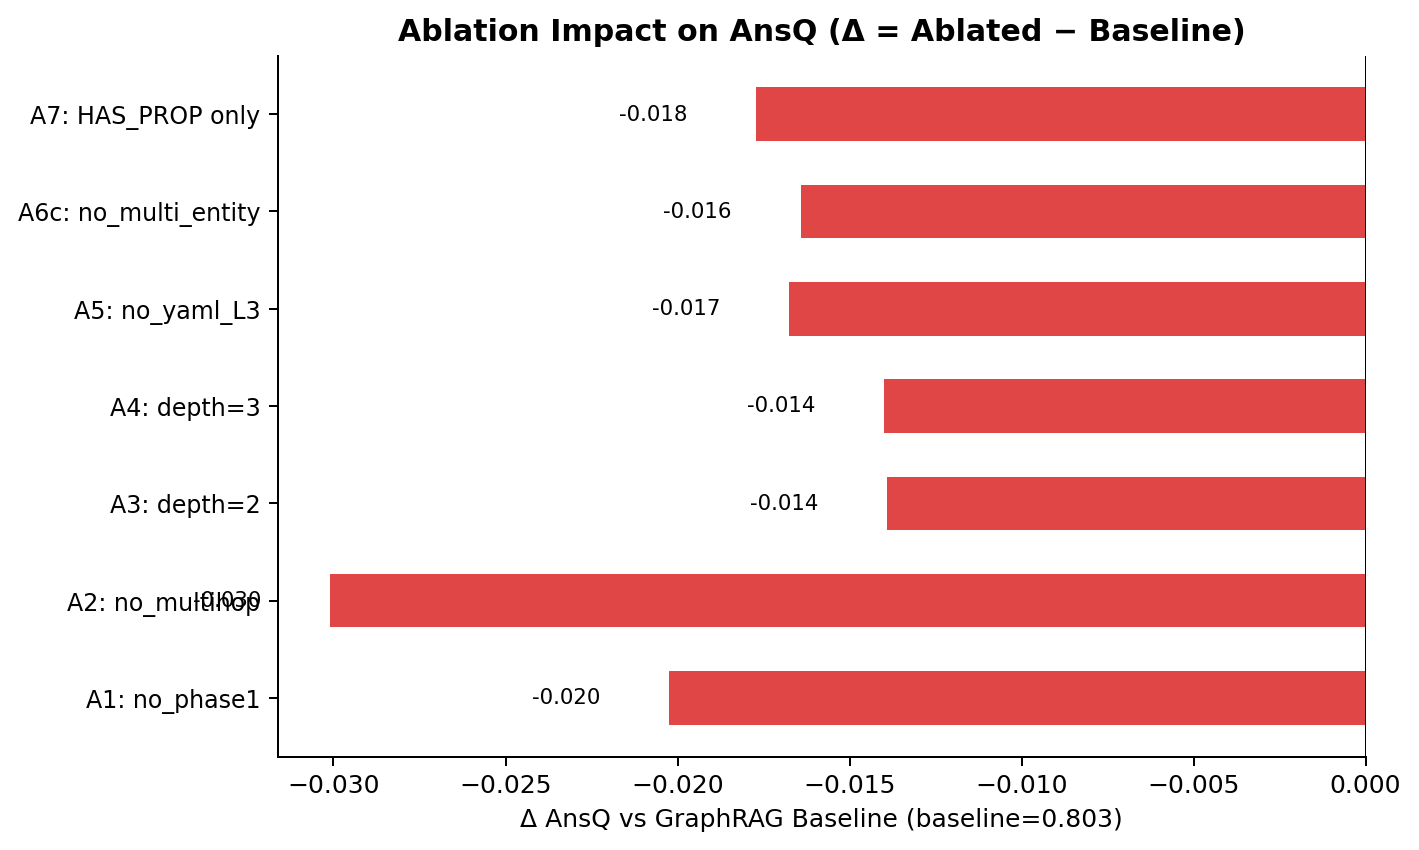
\includegraphics[width=\linewidth]{figures/id/fig2_ablation.png}
    \xfigwd=0pt
    \caption{Penurunan RetQ F1 dan \textit{hop accuracy} pada tiap konfigurasi ablasi relatif terhadap \textit{baseline}.}
    \label{fig:ablasi}
\end{figure}

\subsection{Pembahasan: Faithfulness dan Batas Keunggulan}

\textit{Faithfulness} GraphRAG (0,31) lebih tinggi secara signifikan dibanding Vector RAG (0,17), namun nilai absolutnya berada jauh di bawah ambang ideal. Dekomposisi klaim jawaban mengungkap bahwa sekitar 56\% klaim bersumber dari pengetahuan parametrik LLM, bukan dari konteks graf yang di-\textit{retrieve}. Hal ini bukan cacat sistem, melainkan konsekuensi arsitektural: \textit{knowledge graph} yang dibangun dari blok \textit{definitions} hanya memodelkan relasi antar-\textit{resource} bertipe objek sebagai \textit{edge}, sedangkan nilai atribut skalar (seperti nama kontainer atau \textit{image}) tidak dapat direpresentasikan sebagai simpul graf. Sistem karenanya dirancang \textit{open-book}: LLM diizinkan melengkapi jawaban dengan pengetahuan parametrik ketika informasi tidak tersedia dalam graf. Analisis korelasi menunjukkan \textit{faithfulness} berkorelasi lemah dan tidak signifikan terhadap AnsQ, menegaskan bahwa keduanya mengukur aspek yang berbeda: AnsQ mengukur kebenaran dan relevansi jawaban, sedangkan \textit{faithfulness} mengukur keterlacakan klaim ke konteks yang di-\textit{retrieve}.

Tiga keterbatasan turut membingkai cakupan temuan ini. Pertama, \textit{knowledge graph} yang dibangun bersifat statis dan hanya merepresentasikan relasi struktural-skema dari blok \textit{definitions}; relasi operasional seperti ikatan RBAC hanya terjangkau pada satu arah, dan status \textit{runtime} klaster tidak terepresentasikan. Kedua, \textit{retrieval} dibatasi pada maksimum tiga lompatan sehingga kueri yang membutuhkan konteks di luar jangkauan ini mengandalkan pengetahuan parametrik LLM secara \textit{silent}, dengan kategori \textit{relationship} memperoleh manfaat GraphRAG paling kecil di antara seluruh kategori kendati tetap positif. Ketiga, keunggulan GraphRAG tidak menjangkau seluruh dimensi evaluasi: AnsQ setara dengan Vector RAG, dan \textit{faithfulness} mencerminkan keterbatasan cakupan nilai atribut dalam graf, bukan kegagalan mekanisme \textit{retrieval} itu sendiri.

\section{Kesimpulan}
\label{sec:kesimpulan}

Penelitian ini membangun sistem GraphRAG dengan tiga kontribusi teknis: konstruksi \textit{knowledge graph} deterministik dari skema OpenAPI Kubernetes, mekanisme \textit{retrieval} dengan kedalaman \textit{traversal} adaptif per tipe \textit{intent}, serta validasi struktural YAML tiga lapis berbasis graf sebagai alternatif terhadap \textit{dry-run} klaster aktif. Evaluasi terhadap 102 skenario uji menunjukkan keunggulan GraphRAG yang signifikan pada dimensi \textit{retrieval} (F1 0,71 berbanding 0,24, $\Delta{+}0{,}465$ terhadap Vector RAG) dan penalaran struktural, sementara kualitas teks jawaban tetap setara antarsistem karena ditentukan oleh kapabilitas generatif LLM yang identik. Temuan ini menegaskan bahwa kontribusi representasi graf pada domain konfigurasi Kubernetes terletak pada ketertelusuran dan kelengkapan \textit{retrieval} struktural, bukan pada kefasihan bahasa jawaban.

\section*{Acknowledgment}
Naskah ini disusun dengan bantuan LLM untuk memadatkan teks dari dokumen Tugas Akhir penulis pertama; seluruh klaim teknis, data, dan hasil eksperimen berasal dari penelitian yang telah dilaksanakan dan divalidasi oleh penulis.

\bibliographystyle{IEEEtran}
\bibliography{refs}

\begin{biographynophoto}{Jihan Aurelia}
adalah mahasiswa Program Studi Sistem dan Teknologi Informasi, Institut Teknologi Bandung, dengan fokus penelitian pada representasi pengetahuan berbasis graf untuk sistem \textit{retrieval-augmented generation}.
\end{biographynophoto}

\begin{biographynophoto}{Dimitri Mahayana}
(Dr., Ir., M.Eng.) adalah dosen pembimbing pada Sekolah Teknik Elektro dan Informatika, Institut Teknologi Bandung.\EOD
\end{biographynophoto}

\end{document}
